\documentclass[a4paper, 14pt]{article}

\usepackage{arxiv}

\usepackage[T2A]{fontenc}
\usepackage[utf8]{inputenc}
\usepackage[english, russian]{babel}
% \usepackage{cmap}
\usepackage{url}
\usepackage{booktabs}
\usepackage{nicefrac}
\usepackage{microtype}
\usepackage{lipsum}
\usepackage{graphicx}
\usepackage{subfig}
\usepackage[square,sort,comma,numbers]{natbib}
\usepackage{doi}
\usepackage{multicol}
\usepackage{multirow}
\usepackage{tabulary}

\usepackage{tikz}
\usetikzlibrary{matrix}

% Algorithms
\usepackage{algpseudocode}
\usepackage{algorithm}

%% Шрифты
\usepackage{euscript} % Шрифт Евклид
\usepackage{mathrsfs} % Красивый матшрифт
\usepackage{extsizes} % Возможность сделать 14-й шрифт

\usepackage{makecell} % diaghead in a table
\usepackage{amsmath,amsfonts,amssymb,amsthm,mathtools,dsfont}
\usepackage{icomma}

\newcommand{\bz}{\mathbf{z}}
\newcommand{\bx}{\mathbf{x}}
\newcommand{\by}{\mathbf{y}}
\newcommand{\bv}{\mathbf{v}}
\newcommand{\bw}{\mathbf{w}}
\newcommand{\ba}{\mathbf{a}}
\newcommand{\bb}{\mathbf{b}}
\newcommand{\bff}{\mathbf{f}}
\newcommand{\bh}{\mathbf{h}}
\newcommand{\bg}{\mathbf{g}}
\newcommand{\bl}{\mathbf{l}}
\newcommand{\bp}{\mathbf{p}}
\newcommand{\bq}{\mathbf{q}}
\newcommand{\bs}{\mathbf{s}}
\newcommand{\bt}{\mathbf{t}}
\newcommand{\bu}{\mathbf{u}}
\newcommand{\bT}{\mathbf{T}}
\newcommand{\bX}{\mathbf{X}}
\newcommand{\bZ}{\mathbf{Z}}
\newcommand{\bS}{\mathbf{S}}
\newcommand{\bH}{\mathbf{H}}
\newcommand{\bW}{\mathbf{W}}
\newcommand{\bY}{\mathbf{Y}}
\newcommand{\bU}{\mathbf{U}}
\newcommand{\bQ}{\mathbf{Q}}
\newcommand{\bP}{\mathbf{P}}
\newcommand{\bA}{\mathbf{A}}
\newcommand{\bB}{\mathbf{B}}
\newcommand{\bC}{\mathbf{C}}
\newcommand{\bE}{\mathbf{E}}
\newcommand{\bF}{\mathbf{F}}
\newcommand{\bsigma}{\boldsymbol{\sigma}}
\newcommand{\bomega}{\boldsymbol{\omega}}
\newcommand{\btheta}{\boldsymbol{\theta}}
\newcommand{\bgamma}{\boldsymbol{\gamma}}
\newcommand{\bdelta}{\boldsymbol{\delta}}
\newcommand{\bPsi}{\boldsymbol{\Psi}}
\newcommand{\bpsi}{\boldsymbol{\psi}}
\newcommand{\bxi}{\boldsymbol{\xi}}
\newcommand{\bmu}{\boldsymbol{\mu}}
\newcommand{\bchi}{\boldsymbol{\chi}}
\newcommand{\bzeta}{\boldsymbol{\zeta}}
\newcommand{\blambda}{\boldsymbol{\lambda}}
\newcommand{\beps}{\boldsymbol{\varepsilon}}
\newcommand{\bZeta}{\boldsymbol{Z}}
% mathcal
\newcommand{\cX}{\mathcal{X}}
\newcommand{\cY}{\mathcal{Y}}
\newcommand{\cW}{\mathcal{W}}
\newcommand{\cL}{\mathcal{L}}

\newcommand{\dH}{\mathds{H}}
\newcommand{\dR}{\mathds{R}}
% transpose
\newcommand{\T}{^{\mathsf{T}}}

% \renewcommand{\shorttitle}{\textit{arXiv} Шаблон}
\renewcommand{\epsilon}{\ensuremath{\varepsilon}}
\renewcommand{\phi}{\ensuremath{\varphi}}
\renewcommand{\kappa}{\ensuremath{\varkappa}}
\renewcommand{\le}{\ensuremath{\leqslant}}
\renewcommand{\leq}{\ensuremath{\leqslant}}
\renewcommand{\ge}{\ensuremath{\geqslant}}
\renewcommand{\geq}{\ensuremath{\geqslant}}
\renewcommand{\emptyset}{\varnothing}

\usepackage{hyperref}
% \usepackage[usenames,dvipsnames,svgnames,table,rgb]{xcolor}

\hypersetup{
	unicode=true,
	pdftitle={A template for the arxiv style},
	pdfsubject={q-bio.NC, q-bio.QM},
	pdfauthor={David S.~Hippocampus, Elias D.~Striatum},
	pdfkeywords={First keyword, Second keyword, More},
	colorlinks=true,
	linkcolor=black,        % внутренние ссылки
	citecolor=blue,         % на библиографию
	filecolor=magenta,      % на файлы
	urlcolor=blue           % на URL
}

\graphicspath{{../figures/}}

\usepackage{enumitem} % Для модификаций перечневых окружений

\theoremstyle{definition} % "Определение"
\newtheorem{definition}{Опр.}[section]

\usepackage{etoolbox}

\makeatletter
\expandafter\patchcmd\csname\string\algorithmic\endcsname{\itemsep\z@}{\itemsep=1.5mm}{}{}
\makeatother
\renewcommand{\abstractname}{Аннотация}

\title{Состязательные атаки на нейронные сети для работы с временными рядами}

\author{Владимиров Эдуард \\
	\texttt{vladimirov.ea@phystech.edu} \\
	\And
	Зайцев Алексей \\
	\texttt{a.zaytsev@skoltech.ru}
}
\date{\today}

\begin{document}
	\maketitle
	
	\begin{abstract}
		Существует проблема применения состязательных атак в домене временных рядов, и она заключается в том, что эти атаки очень легко обнаружены. В качестве решения этой задачи предлагается использование различных регуляризаторов, которые обеспечивают сохранение свойств исходного временного ряда. На текущий момент рассмотрен аналог L2-регуляризации. Проведён вычислительный эксперимент с моделями из семейства TS2Vec и с различными датасетами, в котором показано существенное увеличение скрытности атаки.
	\end{abstract}
	
	\keywords{временной ряд \and состязательная атака \and IFGSM}
	
	\section{Введение}
	В работе \cite{vivek2020regularizers} рассмотрено множество модификаций для IFGSM: добавление случайного шума, включение инерции по аналогии с Nesterov Momentum.
	В работе \cite{pialla2023time} используется регуляризатор гладкости.
	В будущем стоит рассмотреть и другие регуляризаторы: на периодичность, на размерность вложения.
	
	\section{Теоретическая часть}

	\subsection{IFGSM}
	$$ \bx_{t+1} = \bx_t + \epsilon \cdot sign \bigl( \nabla_x \cL (\bff_\theta(\bx_t), \by) \bigr) $$
	
	\begin{align*}
		\bh_{t+1} &= \bx_t + \epsilon \cdot sign \bigl( \nabla_x \cL (\bff_\theta(\bx_t), \by) \bigr) \\
		\Delta_{t+1} &= || \bx_0 - \bh_{t+1} || \\
		\bx_{t+1} &= \bx_t + \epsilon_{\max} clip \bigl( \nabla_x \cL (\bff_\theta(\bx_t), \by), -\exp(-\Delta_{t+1}^2), \exp(-\Delta_{t+1}^2) \bigr)
	\end{align*}
	
	
	\section{Постановка задачи}
	Пусть $\bff_\theta: \dR^{E \times T} \longrightarrow [0, 1]$ ~--- обученный классификатор временных рядов, $\bg_\kappa: \dR^{E \times T} \longrightarrow [0, 1]$ ~--- обученный дискриминатор, выдающий вероятность искажения данных.
	Тогда задача поиска 
	
	\section{Вычислительный эксперимент}
	
	\begin{table}[bhtp]
		\caption{Сравнение ванильного и улучшенного IFGSM}
		\begin{tabular}{|l|l|l|l|}
			\hline
			\multicolumn{1}{|c|}{\multirow{2}{*}{Attack}} & \multicolumn{1}{c|}{Dataset} & \multicolumn{1}{c|}{Coffee} & FordA \\ \cline{2-4} 
			\multicolumn{1}{|c|}{}                        & Target model                 & TS2Vec & TS2Vec        \\ \hline
			\multirow{2}{*}{Vanilla IFGSM}                & Effectiveness                & \textbf{1.00}               & \textbf{1.00} \\ \cline{2-4} 
			& Concealability               & 0.08                        & 0.28          \\ \hline
			\multirow{2}{*}{Modified IFGSM}               & Effectiveness                & \textbf{1.00}               & 0.99          \\ \cline{2-4} 
			& Concealability               & \textbf{0.97}               & \textbf{0.92} \\ \hline
		\end{tabular}
	\end{table}
	
	\begin{figure}[bhtp]
		\centering
		\subfloat[Vanilla IFGSM]{%
			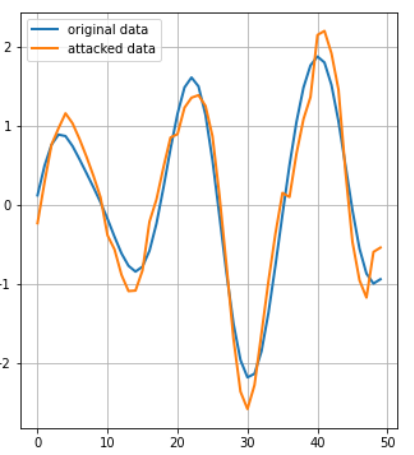
\includegraphics[width=0.48\linewidth]{vanilla-ifgsm}%
		}
		\subfloat[Modified IFGSM]{%
			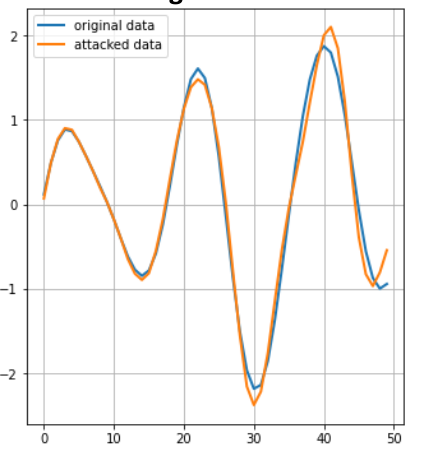
\includegraphics[width=0.48\linewidth]{modified-ifgsm}
		}
		\caption{Визуализация состязательных атак}
		\label{fig:spirals}
	\end{figure}
	
	\section{Заключение}
	TODO
	
	\bibliographystyle{unsrtnat}
	\bibliography{references.bib}
	
\end{document}